%% LyX 2.0.4 created this file.  For more info, see http://www.lyx.org/.
%% Do not edit unless you really know what you are doing.
\documentclass{article}
\usepackage[T1]{fontenc}
\usepackage[latin9]{inputenc}
\usepackage{geometry}
\geometry{verbose,lmargin=2cm,rmargin=2cm}
\usepackage[english]{babel}
\usepackage{graphicx}
\usepackage[unicode=true]
 {hyperref}
\begin{document}
\selectlanguage{english}

\title{Structured Relationship Extraction from Theatrical Works using StageCoach }


\author{Vivek Nair and Dustin A. Janatpou}

\maketitle

\section{Introduction}

Initially, the goal for our project was to extend the social network
extraction research of Elson et. al. on 19th century British fiction
to theatrical works. These works often contain dialogue with attached
attributions, stage directions for specific characters, and other
structured information that allows for the direct creation of social
networks without the use of Named Entity Recognition or extensive
coreference resolution.

However, we quickly realized that there is currently no existing relational
system for storing these works in a way that exploits and represents
this structure. With this in mind, we asked ourselves two fundamental
questions:
\begin{itemize}
\item How feasible is developing a structured, in-memory representation
of the semantic and lexical context of character relationships in
a play? 
\item How could we best construct this system to iteratively test hypotheses
about these relationships?
\end{itemize}
We are currently building a system named StageCoach to answer these
questions. The Github repository for StageCoach can be viewed publicly
at the following URL: <\href{https://github.com/VivekNair/CS224U-StageCoach}{https://github.com/VivekNair/CS224U-StageCoach}>


\section{Previous Approaches}

We primarily draw from Elson et al. (2010)\textquoteright{}s paper\cite{elson2010extracting}
on extracting social networks from 19th Century British fiction. This
approach involves using an \textquotedblleft{}adjacency\textquotedblright{}
metric for relatedness wherein the strength of the relationship between
two characters is determined by the number of words exchanged between
them. We found, however, that the challenge of quote attribution in
narrative fiction was far too complex for the scope of our project.
Instead, we apply some of the network extraction methods discussed
by Elson to theatrical works exactly because these works generally
have built-in quote attribution.

Jing et al. (2007)\cite{jing2007extracting} provides more insight
into constructing these character relationships by specifically mining
dialogue (in the form of interview transcripts) to extract biographical
and relational information. Again, the method\textquoteright{}s performance
is highly reliant on annotation and speaker-role identification (an
equivalent to quote attribution) which is build into the structure
of theatrical works. From here we draw the idea of extracting relations
from dialog directly and using these to weight or declare relationships
between characters.

Other sources of inspiration for developing the system were related
Information Extraction (IE) systems such as KnowItAll and TextRunner,
as described in Etzioni et. al. (2005)\cite{Etzioni200591} and Banko
et. al. (2007)\cite{Banko07openinformation}, respectively. Their
research in providing a structured semantic representation for unstructured
relations gave us the initial idea for constructing a unified representation
of important semantic and lexical elements of the play. 


\section{Current Approach}

\begin{figure}
\caption{\label{fig:1}\protect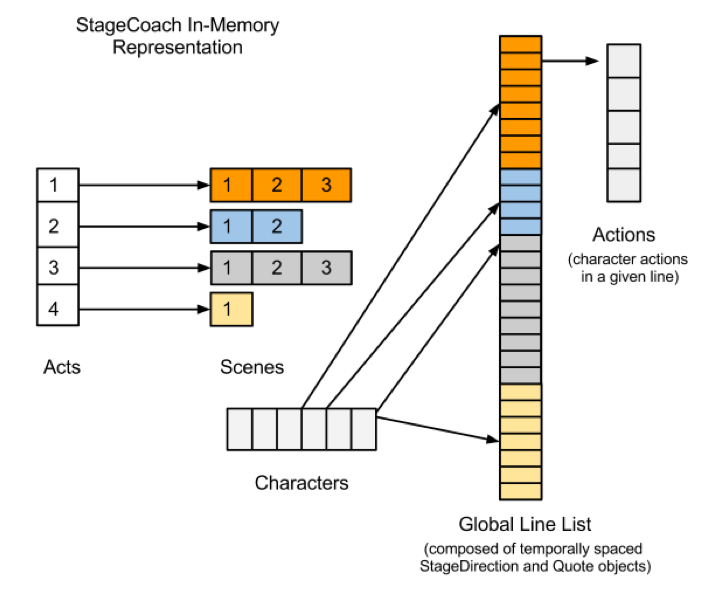
\includegraphics[scale=0.4]{Images/StageCoachInMemory}}
\end{figure}


\begin{figure}
\caption{\label{fig:2}\protect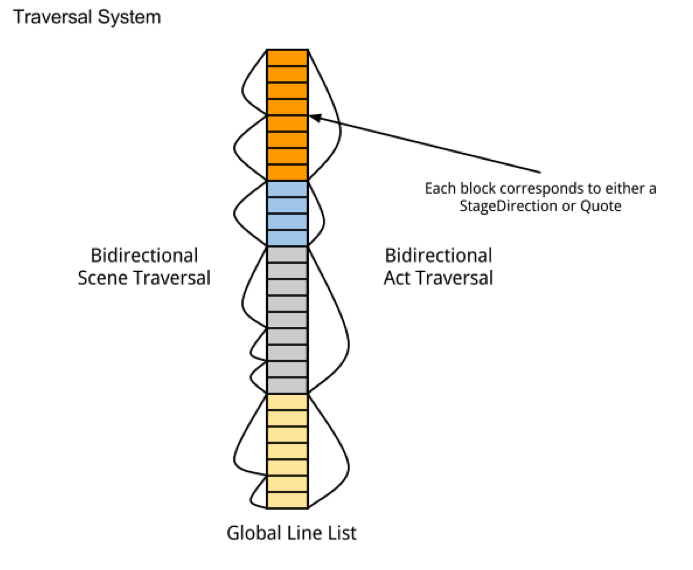
\includegraphics[scale=0.4]{Images/TraversalSystem}}
\end{figure}


\begin{figure}
\caption{\label{fig:3}\protect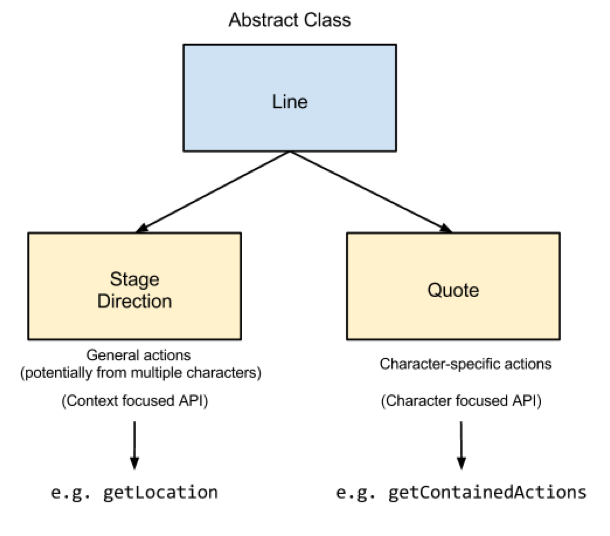
\includegraphics[scale=0.4]{Images/LineClass}}
\end{figure}


\begin{figure}
\caption{\label{fig:4}\protect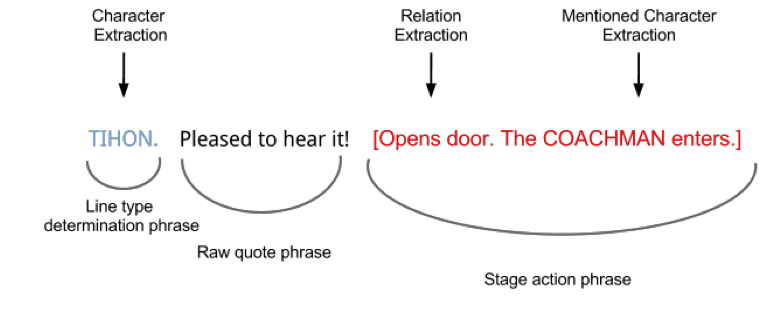
\includegraphics[scale=0.4]{Images/AdditionalExtraction}}
\end{figure}



\subsection{Architecture}

StageCoach {[}see $\mathtt{Figure}$ \ref{fig:1}{]} encapsulates
the fundamental models of a theatrical work in several classes: $\mathtt{StageDirection}$,
$\mathtt{Quote}$, $\mathtt{Character}$, and $\mathtt{Action}$.
The most fundamental unit of representation in our play architecture
is the abstract class $\mathtt{Line}$, from which both $\mathtt{StageDirection}$
and $\mathtt{Quote}$ inherit. Through these two classes, we capture
the distinction between scene-specific and character-specific context
- two ideas which are crucial in understanding the semantic scope
of the theatrical work {[}see $\mathtt{Figure}$ \ref{fig:3}{]}. 

In order to represent temporal segments (e.g. ranges across lines,
scenes, and acts, and arbitrary periods), we have defined an abstract
unit of time $\mathtt{Unit}$ that allows for information extraction
on user-defined units of time (e.g. number of character mentions,
relations for a certain character). We have also started to develop
a traversal architecture that moves between these units of time efficiently
by associating acts and scenes to the Global Line List, a list structure
which holds the entire line-by-line representation of the play. The
conceptual layout of the architecture is partially shown in $\mathtt{Figure}$
\ref{fig:2}.

We have built the basic classes of StageCoach in Java and a preprocessing
script in Ruby, which together allow us to represent Chekhov plays
that conform to the Project Gutenberg format. The Ruby script currently
handles tasks unrelated to the information content of the play; it
removes the Project Gutenberg headers and footers, html tags, newlines,
etc. We will expand this to make plays by other authors conform to
the format our parser expects (by changing \textquotedblleft{}Dramatis
Personae\textquotedblright{} to \textquotedblleft{}CHARACTERS,\textquotedblright{}
for example). We eventually expect to integrate this pre-processing
step into the existing StageCoach architecture. 


\subsection{Network Extraction}

Once we have successfully parsed a given play and stored its information
in the architecture discussed above, we will be able to use a number
of different approaches to generate social networks. Because of the
highly structured nature of plays, we will be able to assume that
the attribution of quotes and stage directions, as well as the mapping
from Lines into Scenes and Scenes into Acts, is nearly completely
correct once we\textquoteright{}ve handled edge cases. This will allow
us to focus solely on comparing and evaluating different methods of
social network generation, rather than on underlying errors which
would otherwise be propagated.

The most basic metric for relatedness in a play is the number of times,
or amount of time, two characters spend on stage together. We\textquoteright{}ll
call this \textquotedblleft{}coappearance\textquotedblright{}; for
theatrical works with multiple scenes, this is readily determined
from our model for each pair of characters. Building off of Elson,
we plan to next try an adjacency-based network generation model, which
looks not for lines spoken in the same scene, but within some specified
word distance from each other.

An extension to this will make use of relation extraction, applied
both to dialogue and to actions/stage directions. We can manually
assign weights to the importance of different types of extracted relations,
or we can use the outputs of other methods to learn which relations
correlate with observed relationships. The relations can be used to
produce continuous weightings on relationship edges, or could be valuable
as annotations placed on the edges generated by other methods.


\subsection{Evaluation}

Our formative evaluation methods will necessarily be qualitative and
manual. We will need to exploit the modularity of our architecture
to run many different social network construction techniques, beginning
with the ``low-hanging fruit'' of very intuitive approaches such
as scene coappearance. As we try new methods, we will use theatrical
works with which we are familiar to establish a set of results that
``looks right'' before testing the methods on other works. 

We will need a gold standard, though, to perform a quantitative, summative
evaluation and determine the success of our work. This will still
need to be manual, as the only gold standard we can hope for is human
understanding of the relationships presented. To do this, we will
select 3 or 4 plays, or perhaps 3 or 4 Acts from plays that we will
use as our test dataset. We can ask annotators to provide \textquotedblleft{}yes\textquotedblright{}
or \textquotedblleft{}no\textquotedblright{} answers regarding whether
each pair of characters has a relationship. We could also ask for
a set of key identifying tags about each character-character relationship
(e.g. mark down if there is a familial relationship, for example).\textquoteright{}

We\textquoteright{}ll then need to measure Cohen's kappa for our annotators
and map our continuously weighted edges to binary labels on each relationship.
With these, we\textquoteright{}ll easily be able to compute precision
and recall over the presence and absence of relationships. For specific
relationships (if we include that approach), we will be much more
interested in recall as long as the lists of labels are short enough
for a user to easily pick out key relationships.


\section{Obstacles}

The first obstacle we have encountered is inconsistent formatting
for certain input plays, an issue which results in incorrect data
representation in StageCoach's parsing system {[}see $\mathtt{Figure}$
\ref{fig:4}{]}. These inconsistencies prevented us from generalizing
the initial parsing steps, but we hope that by expanding the preprocessing
script we can make this critical step fairly robust.

Once we have the data structure fully functional and the parser operating
smoothly, the biggest hurdle will be evaluation, both formative and
summative. In our formative evaluation, it is simply infeasible to
take a thorough quantitative approach for every extraction method
we would like to test. We can personally annotate a few development
examples to use as targets, but in the end we\textquoteright{}ll be
doing a lot of evaluation by inspection to improve our results from
run to run.

\bibliographystyle{plain}
\addcontentsline{toc}{section}{\refname}\nocite{*}
\bibliography{LitReview_Biblio}


\end{document}
